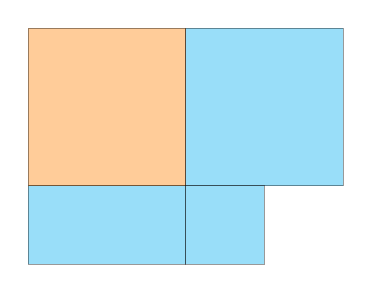
\begin{tikzpicture}
    \coordinate (A) at (0,0);
    \coordinate (B) at (2,0);
    \coordinate (C) at (2,1);
    \coordinate (D) at (0,1);
    \coordinate (E) at (0,3);
    \coordinate (F) at (2,3);
    \coordinate (G) at (4,3);
    \coordinate (H) at (4,1);
    \coordinate (I) at (3,0);
    \coordinate (J) at (3,1);

    \draw[fill = cyan, thin, opacity=0.4] (A) -- (B) -- (C) -- (D) --cycle;
    \draw[fill = orange, thin, opacity=0.4] (D) -- (C) -- (F) -- (E) --cycle;
    \draw[fill = cyan, thin, opacity=0.4] (C) -- (H) -- (G) -- (F) --cycle;
    \draw[fill = cyan, thin, opacity=0.4] (B) -- (I) -- (J) -- (C) --cycle;
\end{tikzpicture}